\begin{figure}[h!]
    \centering
    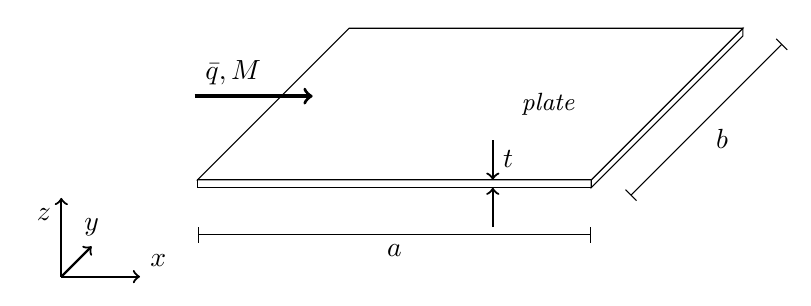
\begin{tikzpicture}
        \draw[thick,->] (-5,-2,-2)  ++(0, 0, 0) -- ++(1, 0, 0) node[anchor=south west] {$x$};
        \draw[thick,->] (-5,-2,-2)  ++(0, 0, 0) -- ++(0, 1, 0) node[anchor=north east] {$z$};
        \draw[thick,->] (-5,-2,-2)  ++(0, 0, 0) -- ++(0, 0, -1) node[anchor=south] {$y$};

        \pgfmathsetmacro{\cubex}{5}
        \pgfmathsetmacro{\cubey}{0.1}
        \pgfmathsetmacro{\cubez}{5}
        
        % \draw[black, fill=white] (2.5,0,0) ++(-\cubex/2+0.25,-\cubey-0.01,0) ++(-0.5,-0.5,0) rectangle ++(0.5,0.5,0);
        % \draw[black, fill=white] (2.5,0,0) ++(-\cubex/2+0.75,-\cubey-0.01,0) ++(-0.5,-0.5,0) -- ++(0.5,0.5,0);
        
        \draw[black, fill=white] (2.5,0,0) -- ++(-\cubex,0,0) -- ++(0,-\cubey,0) -- ++(\cubex,0,0) -- cycle;
        \draw[black, fill=white] (2.5,0,0) -- ++(0,0,-\cubez) -- ++(0,-\cubey,0) -- ++(0,0,\cubez) -- cycle;
        \draw[black, fill=white] (2.5,0,0) -- ++(-\cubex,0,0) -- ++(0,0,-\cubez) -- ++(\cubex,0,0) -- cycle;
        
        \draw[black, |-|] (2.5,-0.7,0) ++(0,0,0) -- ++(-\cubex/2,0,0)node[anchor=north] {$a$} -- ++(-\cubex/2,0,0);
        \draw[black, |-|] (3,-0.2,0) ++(0,0,0) -- ++(0,0,-\cubez/2)node[anchor=north west] {$b$} -- ++(0,0,-\cubez/2);
        
        \draw[black, thick,->] (2.5,0,0)  ++(-\cubex/4,0.5,0)node[anchor=north west]{$t$} -- ++(0,-0.5,0);
        \draw[black, thick,->] (2.5,0,0)  ++(-\cubex/4,-0.5-\cubey,0) -- ++(0,0.5,0);
        
        \draw[black, very thick, ->] (-3.5,0.1,-2.5) ++(0, 0, 0) node[anchor=south west] {$\bar{q}, M$} -- ++(1.5, 0, 0);
        
        % \draw (-1,-.4,0)node[]{\small \emph{stringer}};
        \draw (1,0,-2.5)node[]{\small \emph{plate}};
    \end{tikzpicture}
    \newline
    \caption{Panel dimensions and conditions.}
    \label{fig:problem}
\end{figure}